\documentclass[t, aspectratio=169]{beamer}
\usepackage[utf8]{vietnam}
\usepackage{amsthm,amsmath,amssymb}
\usepackage{lmodern}
\usepackage{booktabs}

% --- MARGIN CONFIG ---
\def\slideContentLeftMargin{0.5cm}
\def\slideContentRightMargin{1cm}
\def\hustHeaderHeight{1cm}
\def\slideContentBotMargin{3.5cm}

\usepackage[blue, 169]{beamerthemeHUST}
\graphicspath{{hust_theme/images/}{figures/}}

\renewcommand{\titlePageTitleX}{-0.5cm}
\renewcommand{\titlePageTitleY}{-0.5cm}
\renewcommand{\hustTitleAlign}{\alignLeft}
\renewcommand{\hustSubtitleAlign}{\alignLeft}
\renewcommand{\hustAuthorAlign}{\alignLeft}
\renewcommand{\hustInstAlign}{\alignLeft}

\title{Chaos Control And Schedule Of Shuttle Buses}
\subtitle{Takashi Nagatani, 2006}
\author{Tran Quang Hung -- 20235502 \\ Le Gia Huy -- 20225498 \\ Nguyen Hoang Son Tung -- 20225536}
\institute{Supervisor: PhD. Bui Quoc Trung \\ Mathematical Modelling -- Hanoi University of Science and Technology}

\begin{document}

\hustintropage{}

\husttitlepage

\begin{frame}{Outline}
	\tableofcontents
\end{frame}

\resetPageCount
\showPageNumber
\useStyleHustFull
\useThinBar

% =====================================================================
\section{Motivation}
% =====================================================================

\begin{frame}{Motivation: The Bus Bunching Problem}
	\begin{columns}[T]
		\begin{column}{0.52\textwidth}
			\small
			\textbf{A familiar phenomenon:}
			\begin{itemize}
				\item Shuttle buses run back and forth between two terminals with no fixed timetable.
				\item Trip duration depends on \textbf{passengers picked up}, which depends on the \textbf{headway} since the previous bus.
			\end{itemize}

			\vspace{0.3em}
			\textbf{The feedback loop $\to$ chaos:}
			\begin{enumerate}
				\item Bus falls behind $\Rightarrow$ more passengers $\Rightarrow$ longer boarding $\Rightarrow$ falls \emph{further} behind.
				\item Next bus finds fewer passengers, speeds up.
				\item Gaps amplify every round $\Rightarrow$ \textbf{deterministic chaos}.
			\end{enumerate}
		\end{column}
		\begin{column}{0.46\textwidth}
			\centering
			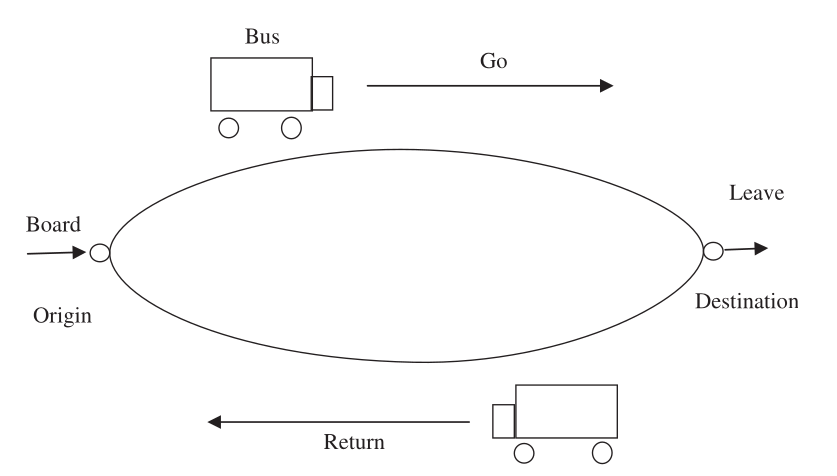
\includegraphics[width=\textwidth,height=5.5cm,keepaspectratio]{fig1_schematic.png}
		\end{column}
	\end{columns}
\end{frame}

% =====================================================================
\section{The Model}
% =====================================================================

\begin{frame}{The Model: Setup and Notation}
	\small
	\begin{columns}[T]
		\begin{column}{0.48\textwidth}
			\textbf{System:} $M$ buses shuttle between Origin and Destination. Passengers board at Origin, alight at Destination.

			\vspace{0.5em}
			\textbf{Key assumptions:}
			\begin{itemize}
				\item Passengers arrive at rate $\mu$ (constant).
				\item Each boarding takes $\gamma$, each alighting takes $\eta$ seconds.
				\item Buses can \emph{overtake} each other.
				\item A delayed bus can \emph{speed up} to compensate.
			\end{itemize}
		\end{column}
		\begin{column}{0.50\textwidth}
			\textbf{Notation:}

			\vspace{0.3em}
			\begin{tabular}{@{}cl@{}}
				\toprule
				Symbol & Meaning \\
				\midrule
				$M$        & number of buses \\
				$t_i(m)$   & arrival time of bus $i$, trip $m$ \\
				$B_i(m)$   & passengers boarding bus $i$ \\
				$V_i(m)$   & average speed of bus $i$ \\
				$\mu$      & passenger arrival rate \\
				$\gamma,\eta$ & board / alight time per pax \\
				$L$        & one-way route length \\
				$V_0$      & base speed (no speedup) \\
				$s_i$      & speedup coefficient of bus $i$ \\
				\bottomrule
			\end{tabular}
		\end{column}
	\end{columns}
\end{frame}

\begin{frame}{The Model: Arrival Time Equation (Eq.~1)}
	A bus trip has three phases: \textbf{arrive} at Origin, \textbf{board/alight} passengers, \textbf{drive} the round trip. So the \emph{next} arrival time is:

	\begin{equation}
		\boxed{\;t_i(m+1) = \underbrace{t_i(m)}_{\text{current time}}
		+ \underbrace{(\gamma + \eta)\,B_i(m)}_{\text{dwell time}}
		+ \underbrace{\frac{2L}{V_i(m)}}_{\text{travel time}}\;}
		\tag{Eq.\,1}
	\end{equation}

	\vspace{0.5em}
	\begin{itemize}
		\item $(\gamma+\eta)\,B_i(m)$: total time spent boarding and alighting passengers.
		\item $\dfrac{2L}{V_i(m)}$: round-trip driving time at average speed $V_i(m)$.
	\end{itemize}

	\vspace{0.3em}
	$\Rightarrow$ We need expressions for $B_i(m)$ and $V_i(m)$ to close this equation.
\end{frame}

\begin{frame}{The Model: Passengers and Speedup (Eq.~2--3)}
	\textbf{Eq.~2 -- Passengers boarding:} proportional to the headway (time since last bus).
	\begin{equation}
		B_i(m) = \mu\,\big(t_i(m) - t_{i'}(m')\big) \equiv \mu\, h_i(m)
		\tag{Eq.\,2}
	\end{equation}
	where $i'$ is whichever bus arrived just before bus $i$, and $h_i(m)$ is the \textbf{headway}.

	\vspace{0.8em}
	\textbf{Eq.~3 -- Speedup control:} a bus with more passengers drives faster to compensate.
	\begin{equation}
		V_i(m) = V_0 + s_i\,(\gamma+\eta)\,B_i(m)
		\tag{Eq.\,3}
	\end{equation}

	\begin{itemize}
		\item $s_i = 0$: no compensation -- speed is always $V_0$.
		\item $s_i$ large: heavy speedup -- the bus tries hard to catch up.
	\end{itemize}

	\vspace{0.3em}
	\alert{Two competing effects:} large headway $\to$ more passengers $\to$ \emph{longer dwell} but also \emph{faster driving}.
\end{frame}

\begin{frame}{The Model: Combined Raw Equation (Eq.~4)}
	Substituting Eq.~2 and Eq.~3 into Eq.~1:
	\begin{equation}
		t_i(m+1) = t_i(m) + \mu(\gamma+\eta)\!\left(t_i(m)-t_{i'}(m')\right) + \frac{2L}{V_0 + s_i\,\mu(\gamma+\eta)\!\left(t_i(m)-t_{i'}(m')\right)}
		\tag{Eq.\,4}
	\end{equation}

	\vspace{0.5em}
	\textbf{Reading this equation:}
	\begin{itemize}
		\item \textbf{Dwell term} $\mu(\gamma+\eta)\,h$: grows linearly with headway $\to$ delays the bus.
		\item \textbf{Travel term} $\frac{2L}{V_0 + s_i\mu(\gamma+\eta)\,h}$: \emph{decreases} with headway $\to$ speeds up the bus.
	\end{itemize}

	\vspace{0.3em}
	$\Rightarrow$ This is a \textbf{nonlinear map}: the next arrival depends on the current headway through both a linear and a reciprocal term. This competition is the source of chaos.
\end{frame}

\begin{frame}{The Model: Dimensionless Map (Eq.~5)}
	\textbf{Non-dimensionalise} by the free-running round-trip time $\tau_0 = 2L/V_0$:
	\[
		T_i \equiv \frac{t_i}{\tau_0}, \qquad
		\Gamma \equiv \mu(\gamma+\eta), \qquad
		S_i \equiv \frac{s_i\,\mu(\gamma+\eta)\cdot 2L}{V_0^2}
	\]

	\vspace{0.2em}
	Defining the \textbf{headway} $H_i(m) \equiv T_i(m) - T_{i'}(m')$, we get:
	\begin{equation}
		\boxed{\;T_i(m+1) = T_i(m) + \Gamma \cdot H_i(m) + \frac{1}{1 + S_i \cdot H_i(m)}\;}
		\tag{Eq.\,5}
	\end{equation}

	\begin{itemize}
		\item $\Gamma$: \textbf{loading parameter} -- how strongly passengers slow the bus.
		\item $S_i$: \textbf{speedup parameter} -- how aggressively bus $i$ compensates.
		\item $H_i$: \textbf{headway} -- the time gap to the previous bus.
	\end{itemize}

	\vspace{0.2em}
	The entire dynamics depend only on $\Gamma$ and $\{S_i\}$ -- all physical constants absorbed.
\end{frame}


% =====================================================================
\section{Methodology}
% =====================================================================

\begin{frame}{Methodology: Simulation Procedure}
	\textbf{Key subtlety:} buses can \emph{overtake} each other, so the ``preceding bus'' in $H_i(m)$ is \textbf{not fixed in advance} -- it depends on the dynamics itself.

	\vspace{0.5em}
	\textbf{Simulation:}
	\begin{enumerate}
		\item Maintain each bus's next arrival time on a priority queue.
		\item Pop the earliest arrival -- that bus has just returned to Origin.
		\item Compute its headway $H_i$ against whichever bus arrived most recently (not a pre-assigned partner).
		\item Apply the nonlinear map (Eq.~5) to compute the next arrival time; push it back onto the queue.
		\item Repeat for all trips; discard the first 900 (transient) and analyse trips 900--1000.
	\end{enumerate}

	\vspace{0.3em}
\end{frame}

% =====================================================================
\section{Results: Time Series}
% =====================================================================

\begin{frame}{Fig. 2 --- Bifurcation Diagrams: Headway vs.\ $\Gamma$}
	\begin{columns}[T]
		\begin{column}{0.55\textwidth}
			\centering
			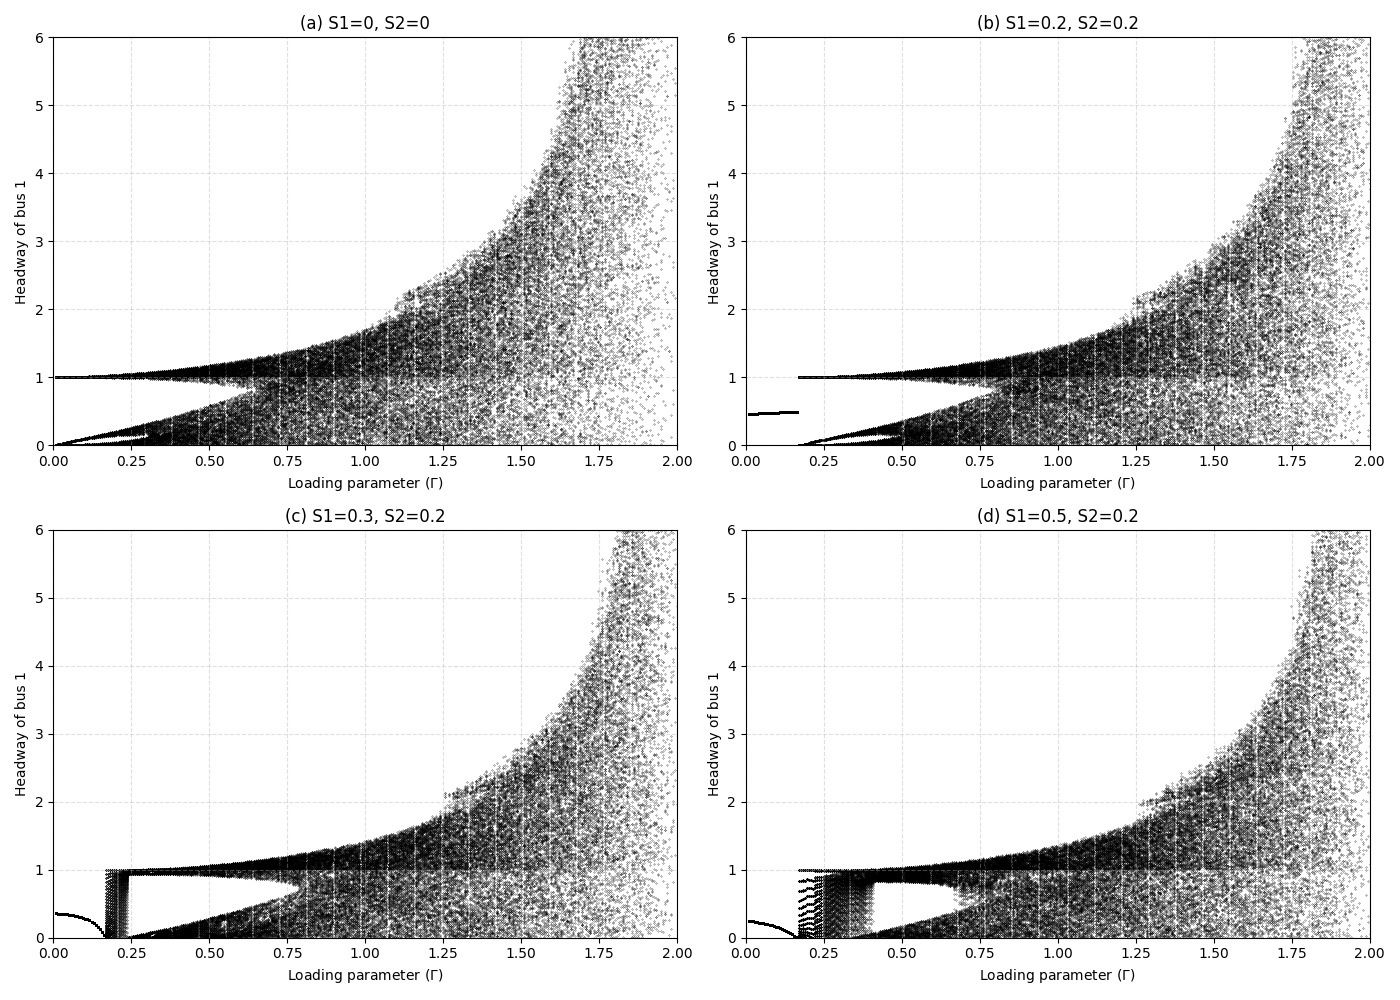
\includegraphics[width=\textwidth]{fig2_time_headway.png}
		\end{column}
		\begin{column}{0.43\textwidth}
			\small
			\begin{itemize}
				\item \textbf{(a) $S_1=S_2=0$:} fluctuation starts at $\Gamma\to0$ -- \alert{no regular regime at all}. Without speedup there is zero stability margin.
				\item \textbf{(b) $S_1=S_2=0.2$:} headway is \emph{exactly} constant until $\Gamma\approx0.167$, then bifurcates.
				\item \textbf{(c)/(d) unequal $S$:} same bifurcation point, but a visibly wider fan of periodic branches first.
				\item All panels share the same shape: a triangular cloud whose \emph{width} grows roughly linearly with $\Gamma$ -- variability, not just the mean, gets worse with load.
			\end{itemize}
		\end{column}
	\end{columns}
\end{frame}

\begin{frame}{Fig. 3 --- Zoom: Period-Adding Route to Chaos}
	\begin{columns}[T]
		\begin{column}{0.55\textwidth}
			\centering
			
\includegraphics[width=\textwidth]{fig3_zoom.png}
		\end{column}
		\begin{column}{0.43\textwidth}
			\footnotesize
			\begin{itemize}
				\item At $\Gamma=0.167$ the constant headway splits into a periodic orbit whose period grows by \emph{addition}: $3\to5\to7\to\ldots$
				\item This is \textbf{period-adding}, \emph{not} period-doubling ($2\to4\to8$) -- a different, less commonly taught route to chaos.
				\item By $\Gamma\approx0.248$ the orbits dissolve into a dense chaotic band.
				\item Panel (b) shows a short \emph{isolated} window of regularity right after the first bifurcation, before the wider chaotic band develops -- the kind of regularity window familiar from the logistic map.
				\item Panel (a) ($S=0$): the fan starts at $\Gamma\to0$ itself, confirming no stability margin without speedup.
			\end{itemize}
		\end{column}
	\end{columns}
\end{frame}

\begin{frame}{Fig. 4 --- Tour-Time Dynamics: Overcompensation}
	\begin{columns}[T]
		\begin{column}{0.55\textwidth}
			\vspace{2.5cm}
			\centering
			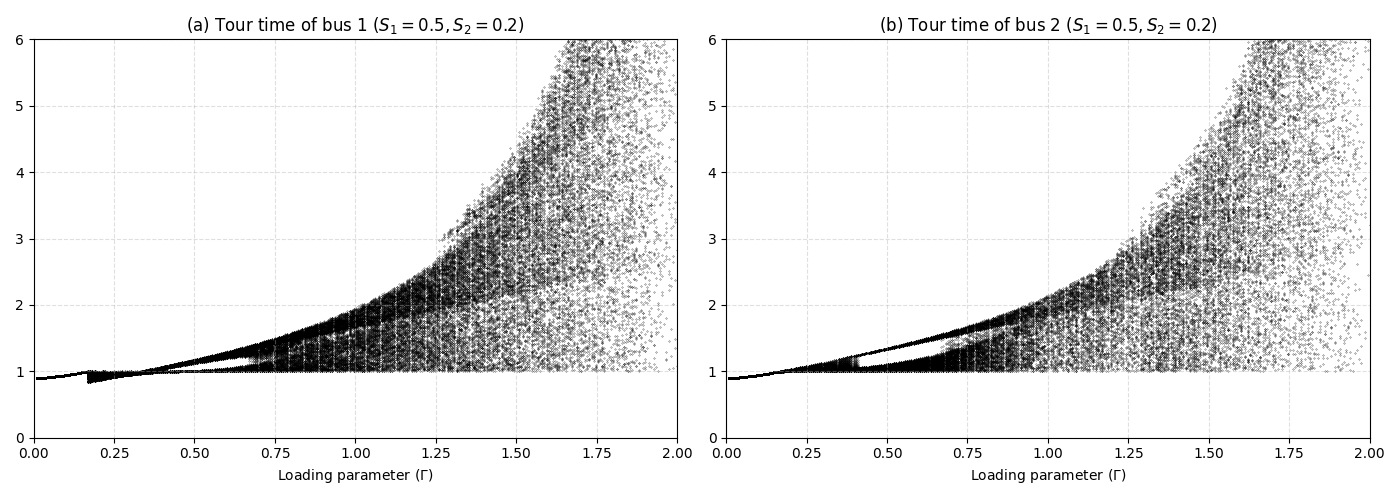
\includegraphics[width=\textwidth]{fig4_tour_time.png}
		\end{column}
		\begin{column}{0.43\textwidth}
			\footnotesize
			\begin{itemize}
				\item Both buses ($S_1=0.5,\ S_2=0.2$) share identical tour time until $\Gamma=0.167$.
				\item Past that point, \textbf{Bus 1} (stronger speedup) fluctuates with \emph{larger} amplitude: a big headway triggers a big speed-up, which \emph{overshoots} and produces a small headway next trip.
				\item Bus 2 (weaker speedup) reacts less aggressively, so it stays more constrained -- at first.
				\item Past $\Gamma\approx0.333$ the two buses \textbf{swap roles}: Bus 2 becomes the more erratic one. The buses are coupled through headway but respond very differently because $S_1\neq S_2$.
			\end{itemize}
		\end{column}
	\end{columns}
\end{frame}

\begin{frame}{Fig. 5 --- Tour-Time Zoom: Coupled Breakdown}
	\begin{columns}[T]
		\begin{column}{0.55\textwidth}
			\vspace{2.5cm}
			\centering
			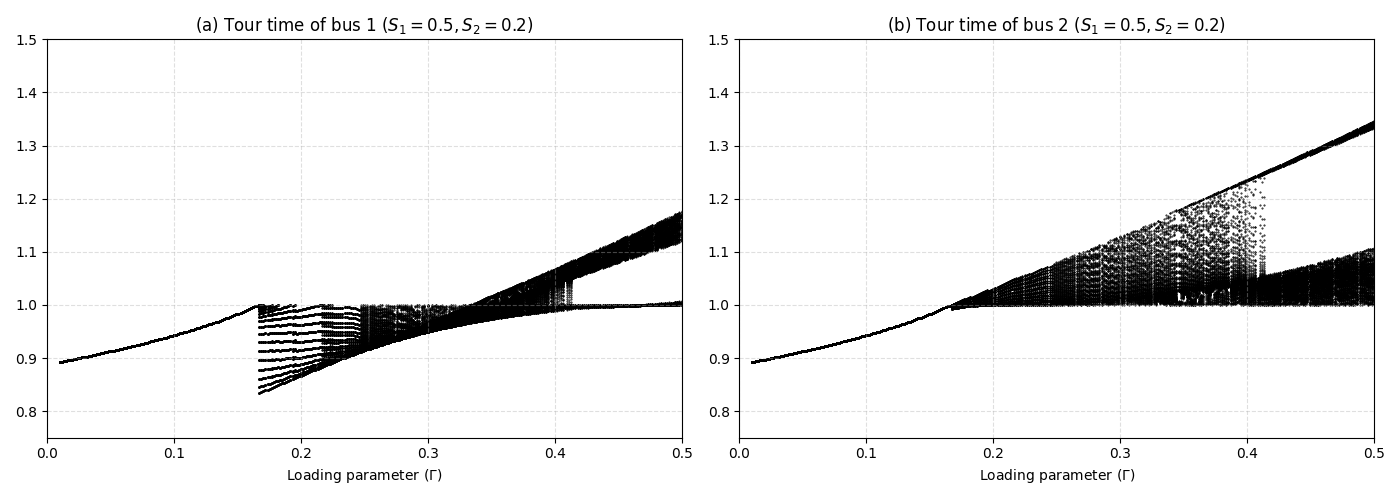
\includegraphics[width=\textwidth]{fig5_zoom.png}
		\end{column}
		\begin{column}{0.43\textwidth}
			\small
			\begin{itemize}
				\item The transition points visible here line up \emph{exactly} with the headway bifurcation points of Fig.~3.
				\item This confirms the schedule breakdown is a single coupled event: the spacing between buses (headway) and the duration of each bus's own trip (tour time) destabilise \textbf{simultaneously}, not independently.
				\item Tour time is therefore not an independent symptom -- it is mechanically tied to headway through the map itself (Eq.~5).
			\end{itemize}
		\end{column}
	\end{columns}
\end{frame}

% =====================================================================
\useStyleLogoOnly
\useThickBar
\section{Results: Phase-Space Analysis}
% =====================================================================

\begin{frame}{Fig. 6 --- Return Maps: Deterministic Structure}
	\begin{columns}[T]
		\begin{column}{0.55\textwidth}
			\centering
			
\includegraphics[width=0.85\textwidth]{fig6_return_map.png}
		\end{column}
		\begin{column}{0.45\textwidth}
			\footnotesize
			\setlength{\itemsep}{0pt}
			\begin{itemize}
				\item \textbf{$\Gamma=0.2$:} 11 points -- \textbf{period-11}, matching Fig.~3's sequence.
				\item \textbf{$\Gamma=0.3$:} piecewise-linear curve; ascending slope $>1$ -- sensitive dependence on initial conditions.
				\item \textbf{$\Gamma=0.5$:} curve splits into \emph{multiple} branches.
				\item \textbf{$\Gamma=0.8$:} many crossing strands -- each bifurcation folds the map again.
				\item Structured curve, not a scattered cloud: proof of \alert{deterministic} chaos, not noise.
			\end{itemize}
		\end{column}
	\end{columns}
\end{frame}

\begin{frame}{Fig. 7 --- Mean and RMS: Three Transition Points}
	\begin{columns}[T]
		\begin{column}{0.55\textwidth}
			\centering
			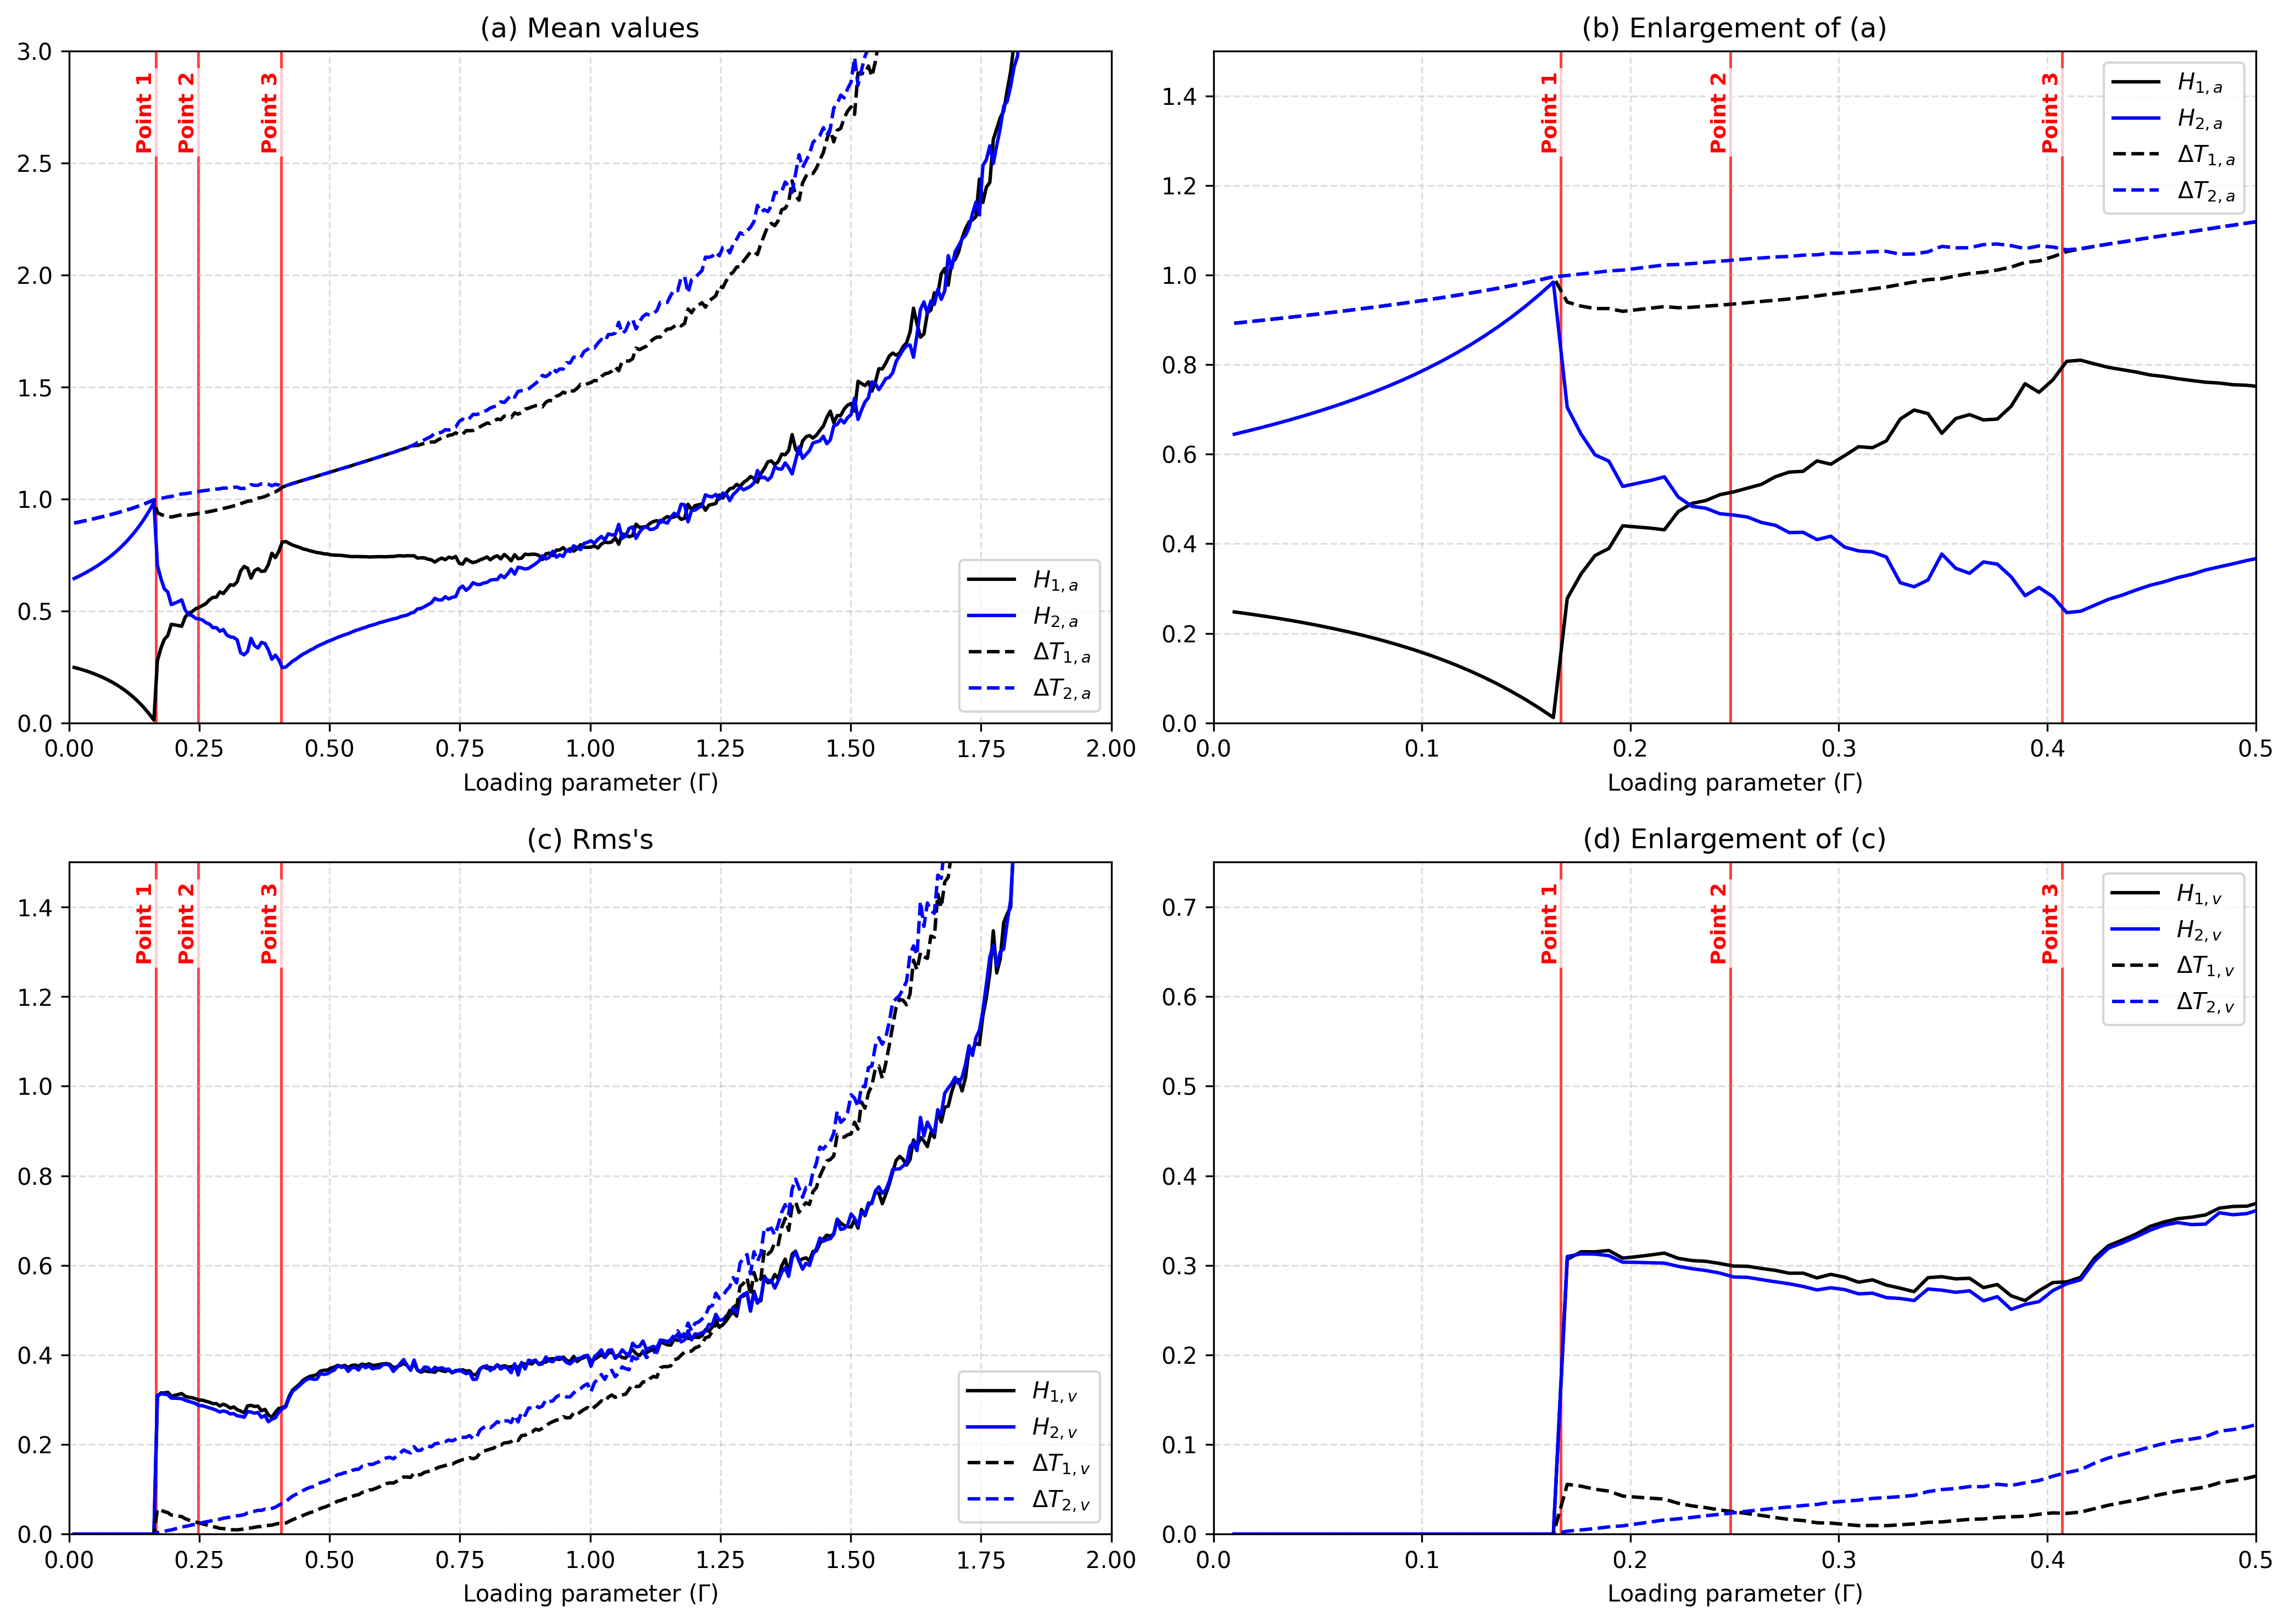
\includegraphics[width=0.95\textwidth]{fig7_mean_rms.png}
		\end{column}
		\begin{column}{0.45\textwidth}
			\footnotesize
			\begin{itemize}
				\item \textbf{Point 1} ($\Gamma\approx0.167$): RMS leaves zero -- onset of non-regular motion.
				\item Just past Point 1, mean headway of Bus~2 (weak speedup) \emph{drops} toward zero while Bus~1's \emph{rises} -- Bus~2 is, on average, closer to bunching with its predecessor.
				\item \textbf{Point 2} ($\Gamma\approx0.333$): the two means \emph{cross} -- the buses swap roles (matches Fig.~4).
				\item \textbf{Point 3:} local minimum of tour-time RMS, after which both buses' variability grows monotonically toward the $\Gamma=2$ divergence.
				\item Full-range panels (a)/(c) show narrow resonance spikes above $\Gamma\approx1.3$ -- brief re-synchronisation into low-period orbits before chaos resumes.
			\end{itemize}
		\end{column}
	\end{columns}
\end{frame}

\begin{frame}{Fig. 8 --- Phase Diagram: Where Speedup Helps}
	\begin{columns}[T]
		\begin{column}{0.55\textwidth}
			\centering
			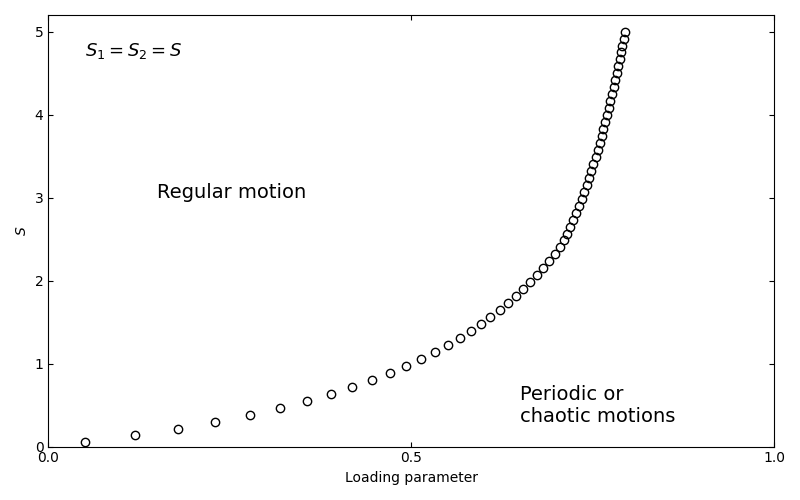
\includegraphics[width=0.95\textwidth]{fig8_phase_diagram.png}
		\end{column}
		\begin{column}{0.45\textwidth}
			\footnotesize
			\setlength{\itemsep}{0pt}
			\begin{itemize}
				\item Symmetric case $S_1=S_2=S$: a critical loading $\Gamma^*(S)$ separates \textbf{regular} (above) from \textbf{periodic/chaotic} (below).
				\item No closed-form $\Gamma^*(S)$ exists -- determined \textbf{numerically} by bisection search.
				\item Convex curve: each extra unit of speedup buys a \emph{smaller} gain in safe loading at low $S$, then steepens above $S\approx2$.
				\item \alert{Diminishing returns aren't the whole story} -- our own search finds the curve cannot rise forever (see $M=3$ section).
			\end{itemize}
		\end{column}
	\end{columns}
\end{frame}

% =====================================================================
\useStyleHustFull
\useThinBar
\section{Extension: Three Buses}
% =====================================================================

\begin{frame}{Generalising Beyond $M=2$}
	\footnotesize
	The paper studies only $M=2$ buses. Our event-driven simulator never assumed $M=2$ -- at each step, the popped bus's predecessor is simply whichever bus arrived most recently, regardless of how many buses exist.

	\vspace{0.3em}
	\alert{No new model is needed for $M=3$:} the exact same map $T_i(m{+}1)=T_i(m)+\Gamma H_i(m)+\frac{1}{1+S_i H_i(m)}$ is applied verbatim -- only the predecessor $i'$ is now chosen among \emph{two} other buses instead of one.

	\vspace{0.3em}
	\textbf{What we made fully general (code):}
	\begin{itemize}
		\setlength{\itemsep}{0pt}
		\item \texttt{simulate(G, S, M, ...)} already accepted arbitrary $M$ -- no change needed.
		\item A single \texttt{bifurcation\_sweep(M, S, Gs, ...)} helper now drives every bifurcation figure, for $M=2$ \emph{or} $M=3$.
		\item Interactive demo: parameter panel and return-map grid generated dynamically for any $M\in[2,8]$.
	\end{itemize}

	\vspace{0.2em}
	\textbf{Question:} does adding a third bus make chaos better or worse?
\end{frame}

\begin{frame}{Three Speedup Cases for $M=3$}
	\footnotesize
	We mirror the three key $M=2$ cases from Fig.~2, with a third bus inserted: \textbf{Case A} $S=(0,0,0)$ (cf.\ Fig.~2a), \textbf{Case B} $S=(0.2,0.2,0.2)$ (cf.\ Fig.~2b), \textbf{Case C} $S=(0.5,0.3,0.2)$ (cf.\ Fig.~2d).

	\vspace{0.2em}
	\begin{columns}[T]
		\begin{column}{0.5\textwidth}
			\centering
			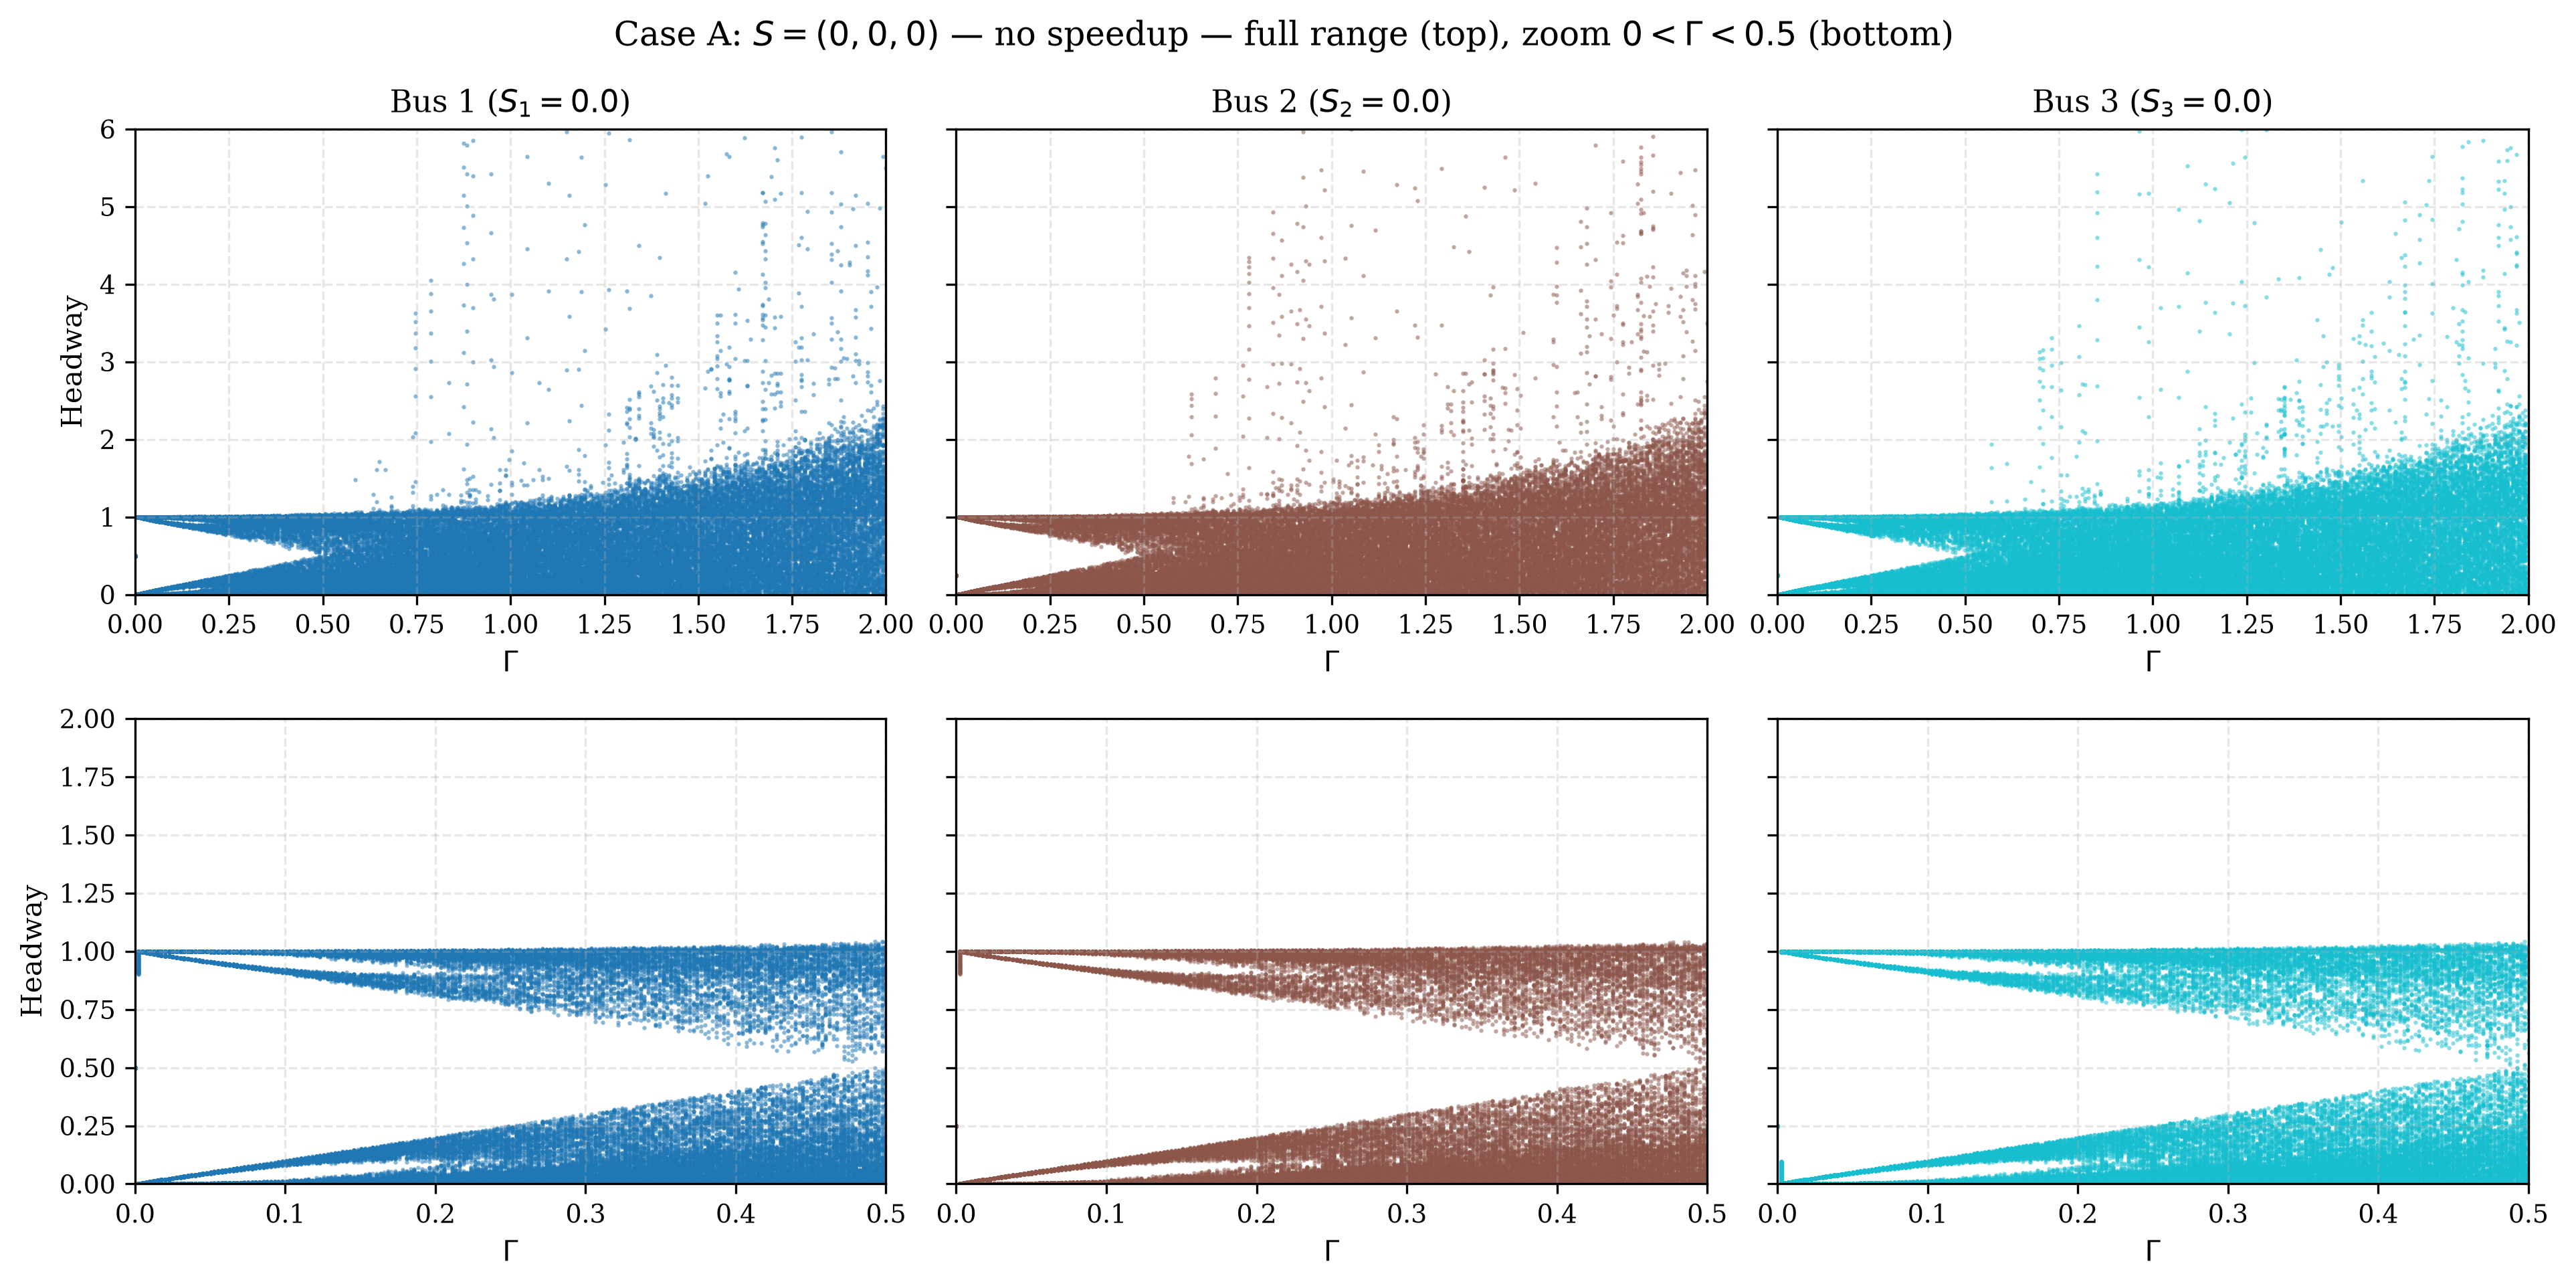
\includegraphics[width=\textwidth,height=4.6cm,keepaspectratio]{fig9a_three_bus_S0.png}\\
			\footnotesize Case A: chaos from $\Gamma\to0$, just like $M=2$.
		\end{column}
		\begin{column}{0.5\textwidth}
			\centering
			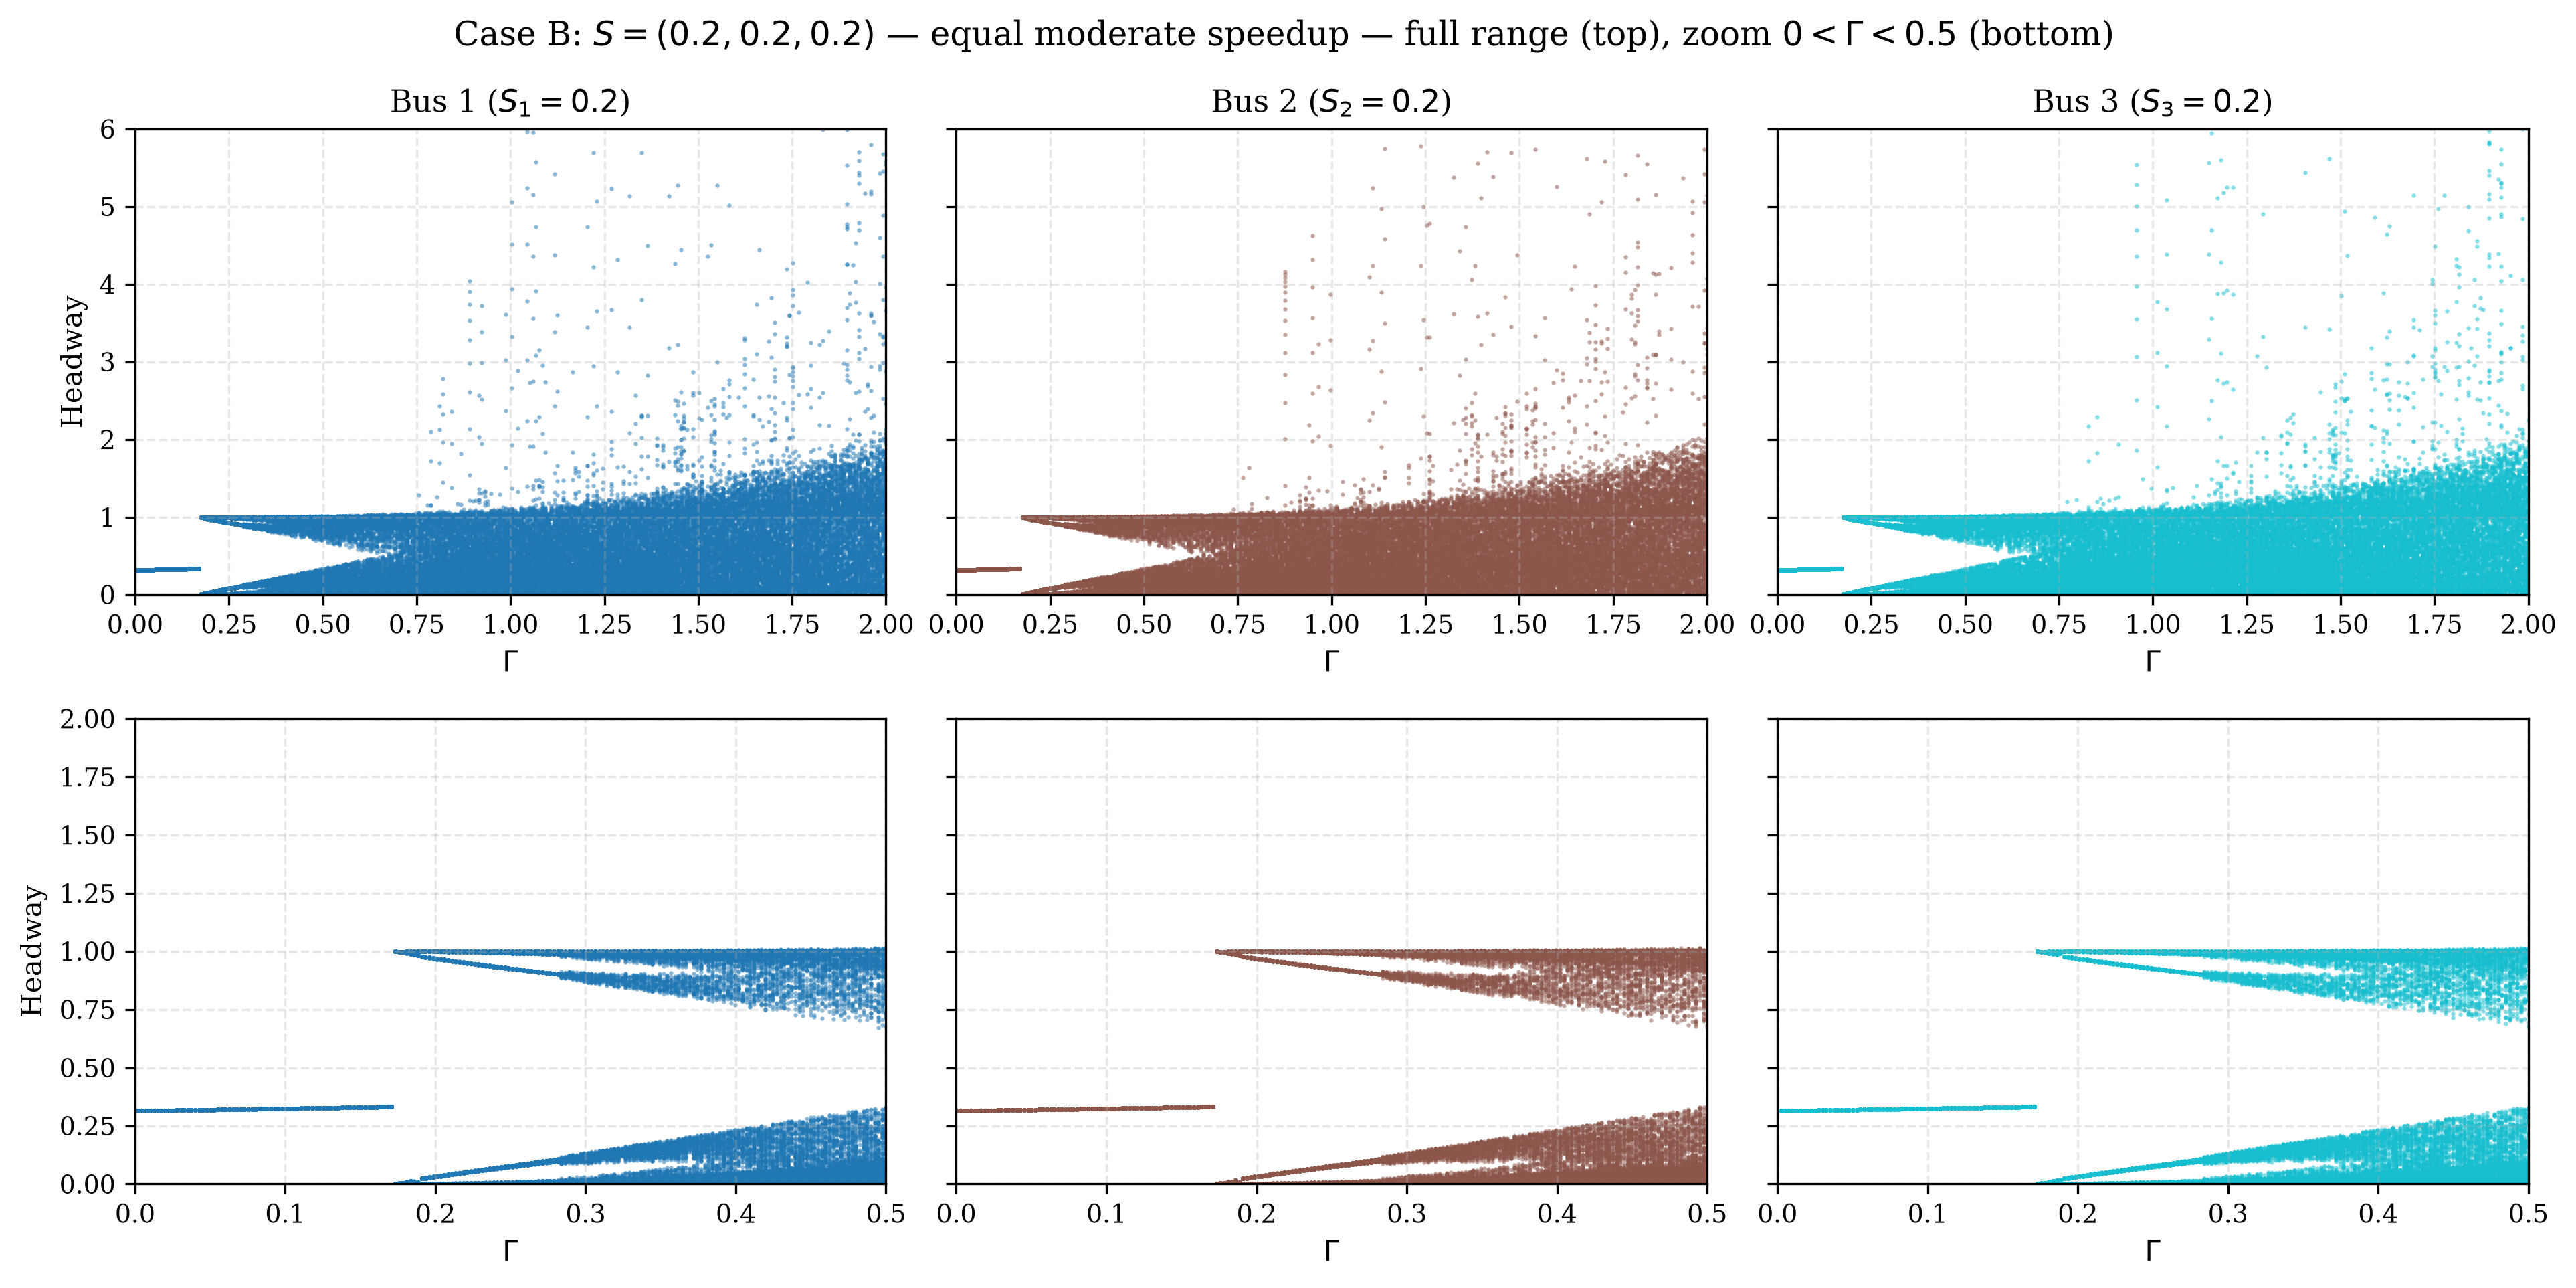
\includegraphics[width=\textwidth,height=4.6cm,keepaspectratio]{fig9b_three_bus_S0.2.png}\\
			\footnotesize Case B: shared, symmetric bifurcation point.
		\end{column}
	\end{columns}
\end{frame}

\begin{frame}{Case C: Graded Speedup with Three Buses}
	\begin{columns}[T]
		\begin{column}{0.55\textwidth}
			\vspace{2cm}
			\centering
			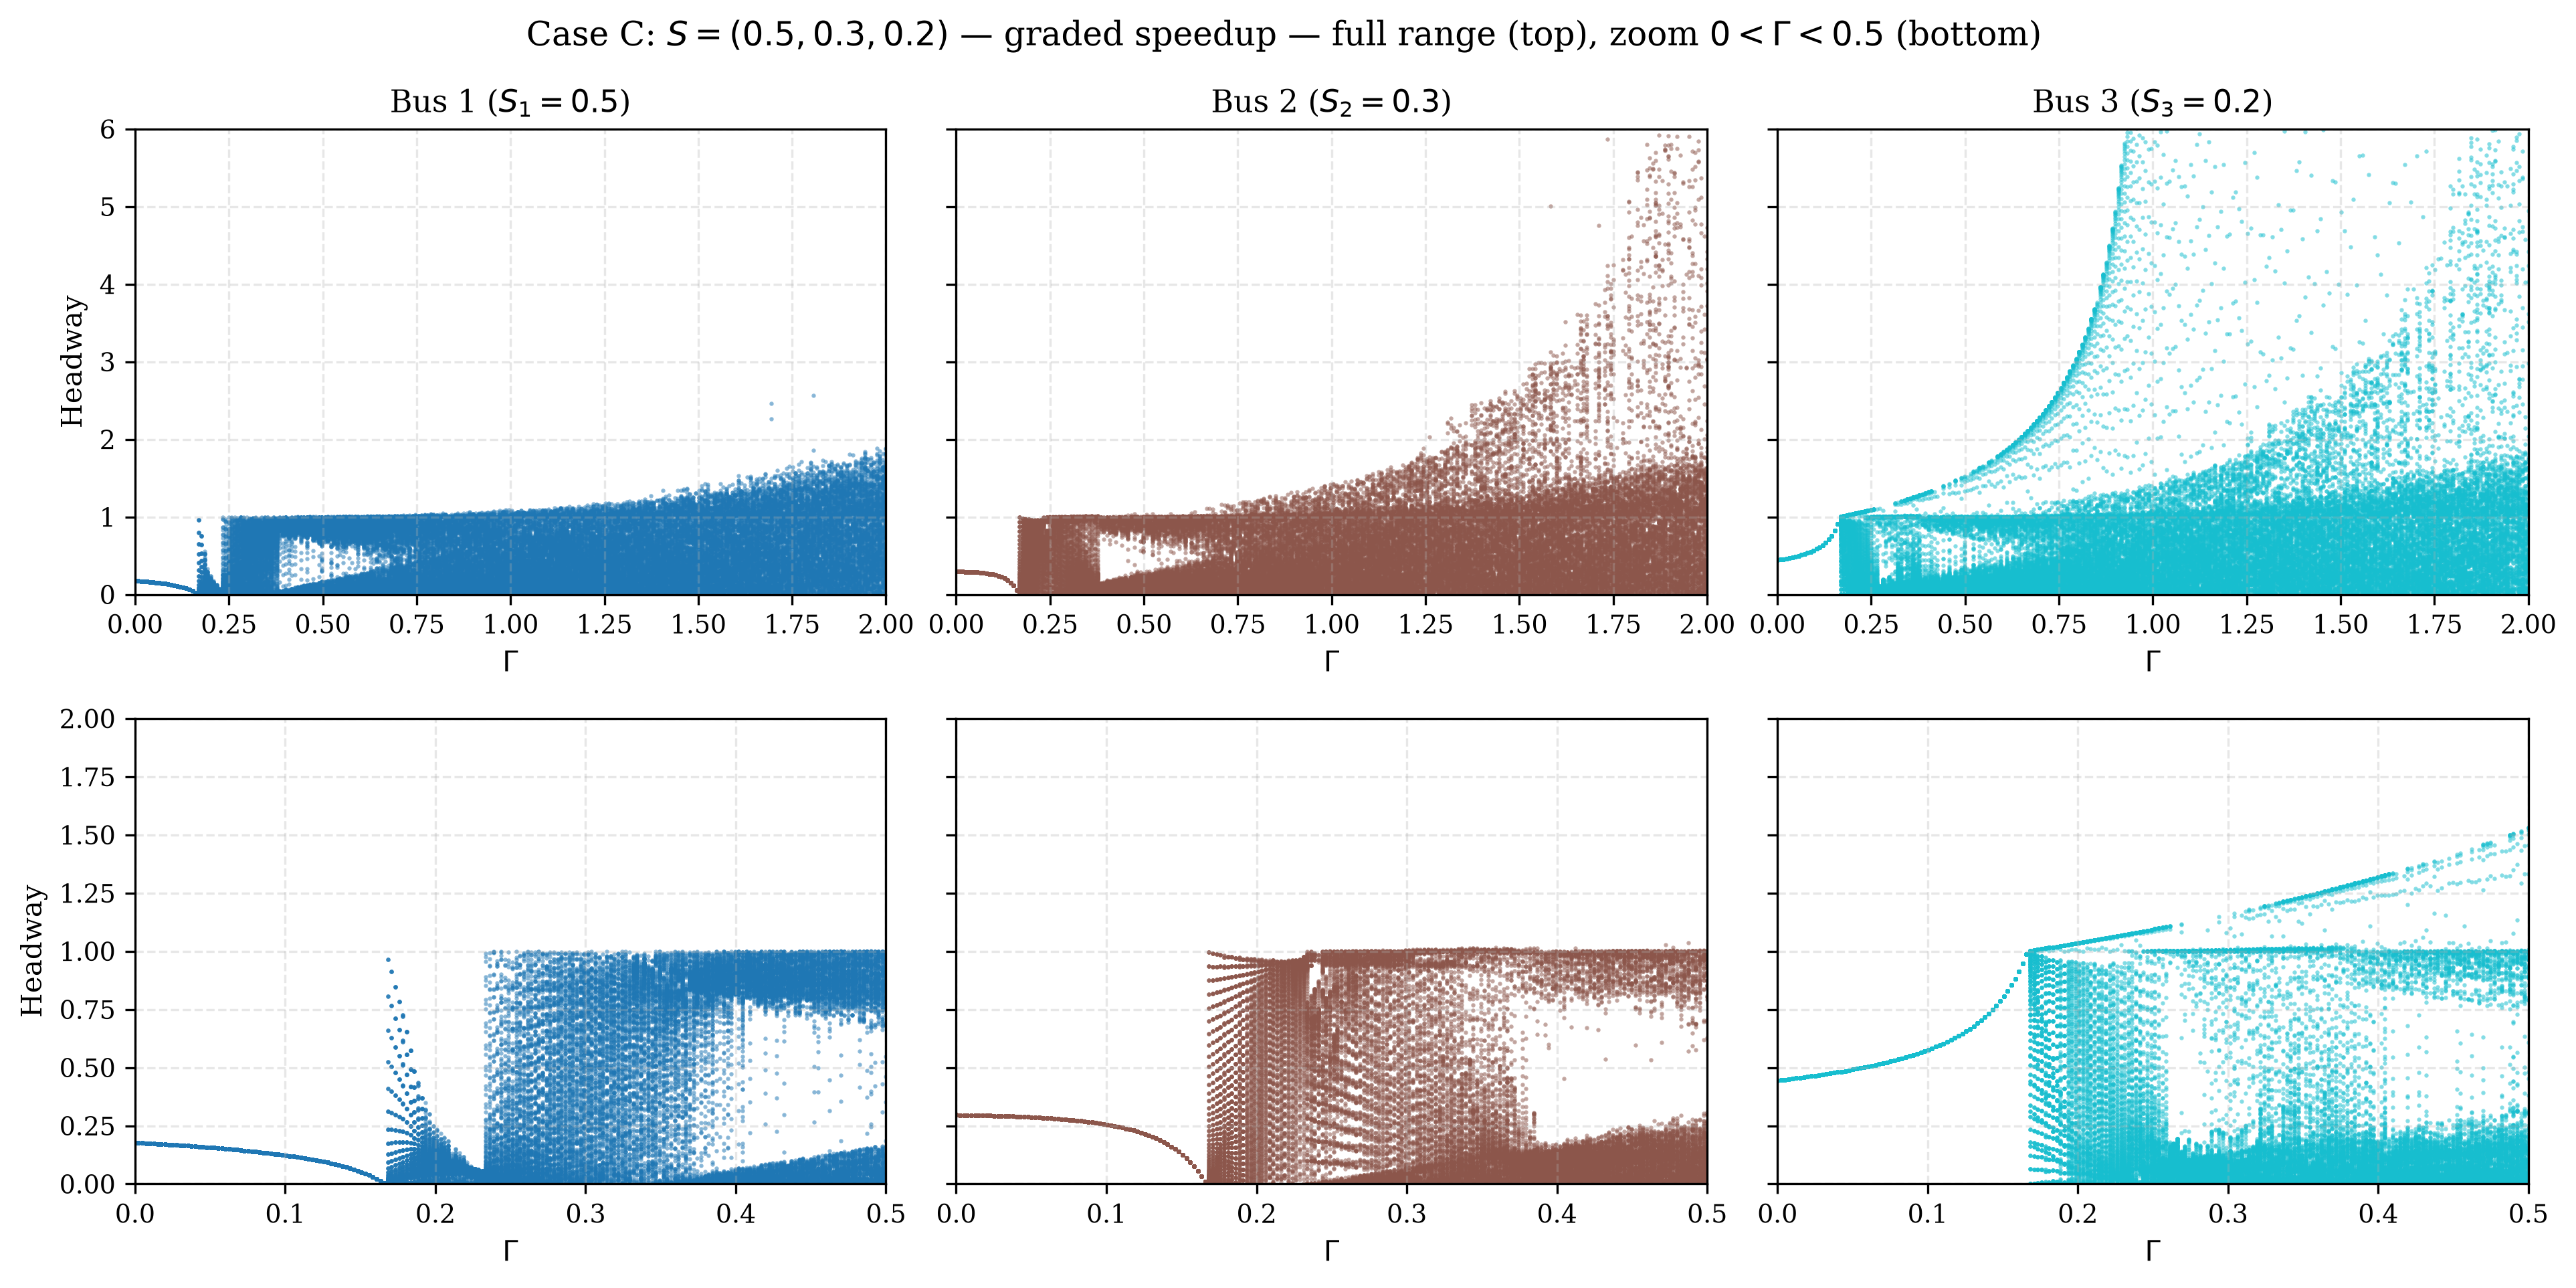
\includegraphics[width=\textwidth]{fig9c_three_bus_graded.png}
		\end{column}
		\begin{column}{0.43\textwidth}
			\small
			\begin{itemize}
				\item Same period-adding route to chaos as $M=2$; the weakest-speedup bus ($S_3=0.2$) is the most violent at high $\Gamma$, just like Bus~2 was before.
				\item All three buses bifurcate near $\Gamma\approx0.15$--$0.2$: chaos onset is a property of the \emph{whole coupled system}, not any single bus.
				\item \alert{Quantitatively:} $\Gamma^*(M{=}3,S{=}0.2)=0.173$ vs.\ $\Gamma^*(M{=}2,S{=}0.2)=0.169$ -- a third bus delays chaos by less than $0.005$ in $\Gamma$. Essentially negligible at moderate speedup.
			\end{itemize}
		\end{column}
	\end{columns}
\end{frame}

\begin{frame}{Fig. 10 --- Return Maps Become Two-Valued}
	\begin{columns}[T]
		\begin{column}{0.55\textwidth}
			\centering
			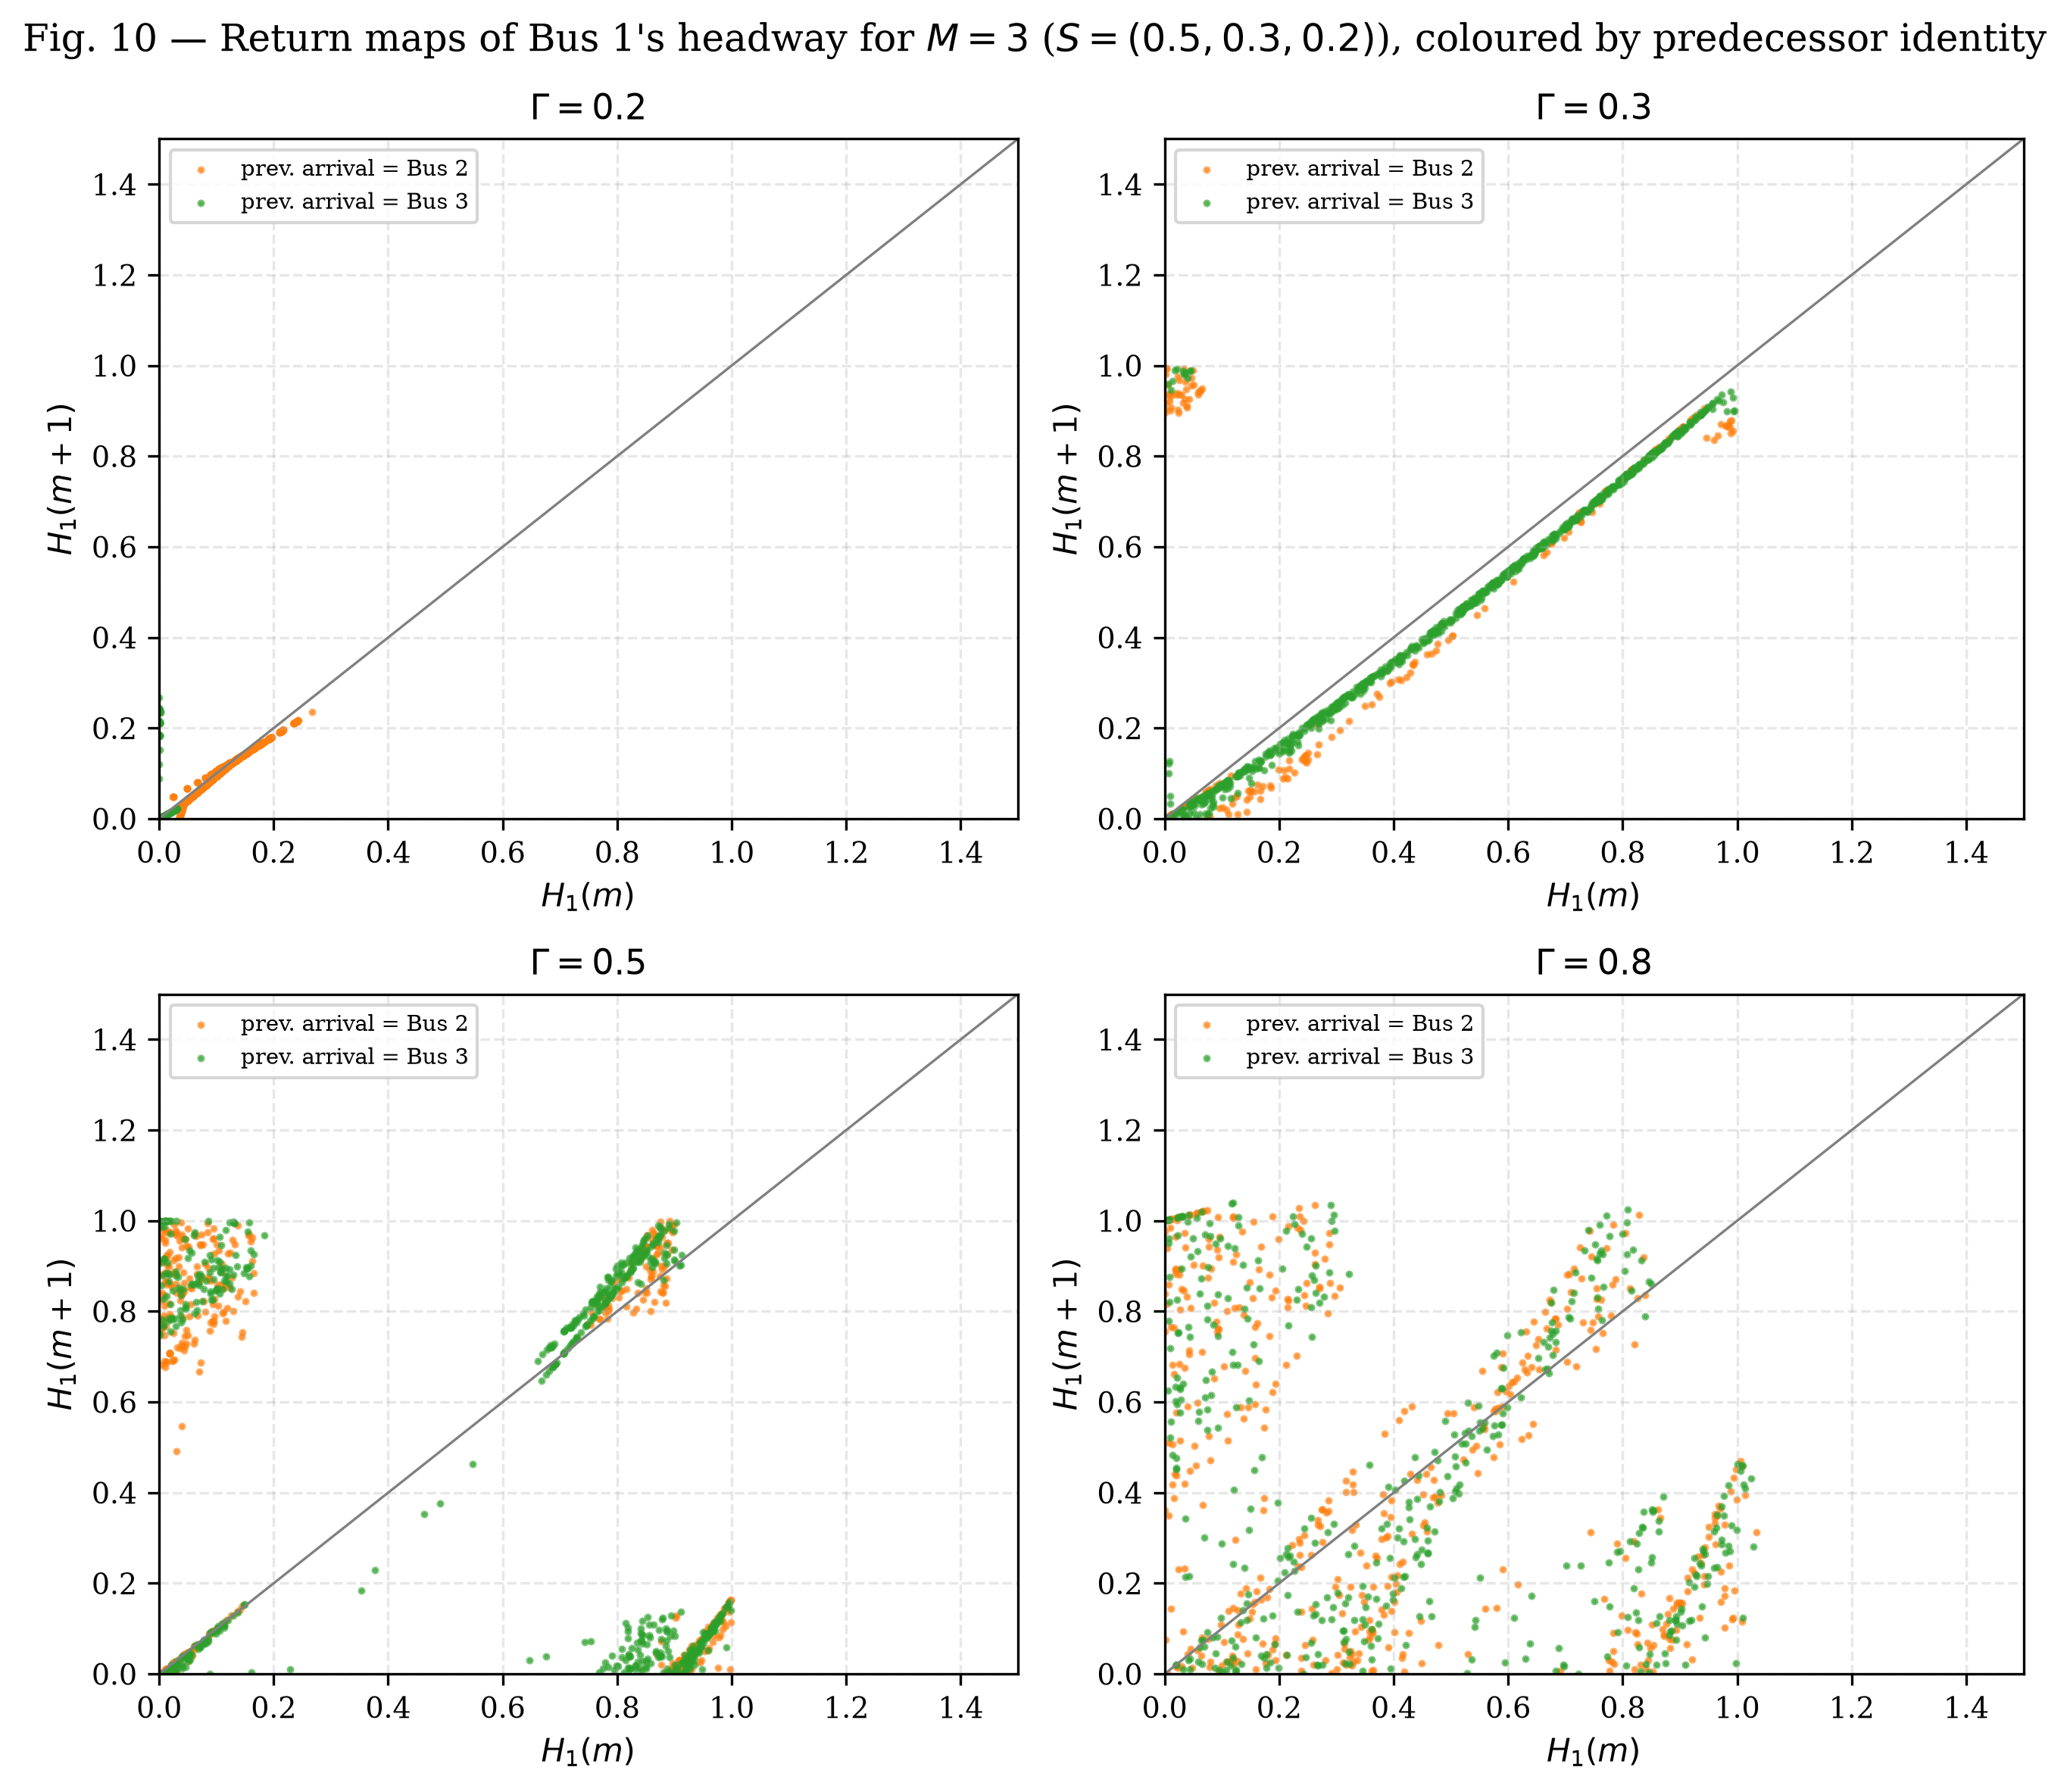
\includegraphics[width=0.8\textwidth]{fig10_three_bus_returnmap.png}
		\end{column}
		\begin{column}{0.43\textwidth}
			\footnotesize
			\begin{itemize}
				\item With $M=2$, a bus has exactly \emph{one} possible predecessor, so its return map is a clean function of $H(m)$ alone.
				\item With $M=3$, Bus~1's predecessor alternates between Bus~2 and Bus~3. Colouring each point by predecessor identity reveals the structure.
				\item At low $\Gamma$ the two predecessor branches (orange/green) overlap almost perfectly.
				\item At high $\Gamma$ they \textbf{visibly separate}: the \emph{same} $H_1(m)$ can map to \emph{different} $H_1(m{+}1)$ depending on who arrived just before.
				\item Still fully deterministic, but the attractor genuinely lives in a higher-dimensional space than $M=2$.
			\end{itemize}
		\end{column}
	\end{columns}
\end{frame}

\begin{frame}{Fig. 11 --- The Speedup Ceiling}
	\begin{columns}[T]
		\begin{column}{0.62\textwidth}
			\centering
			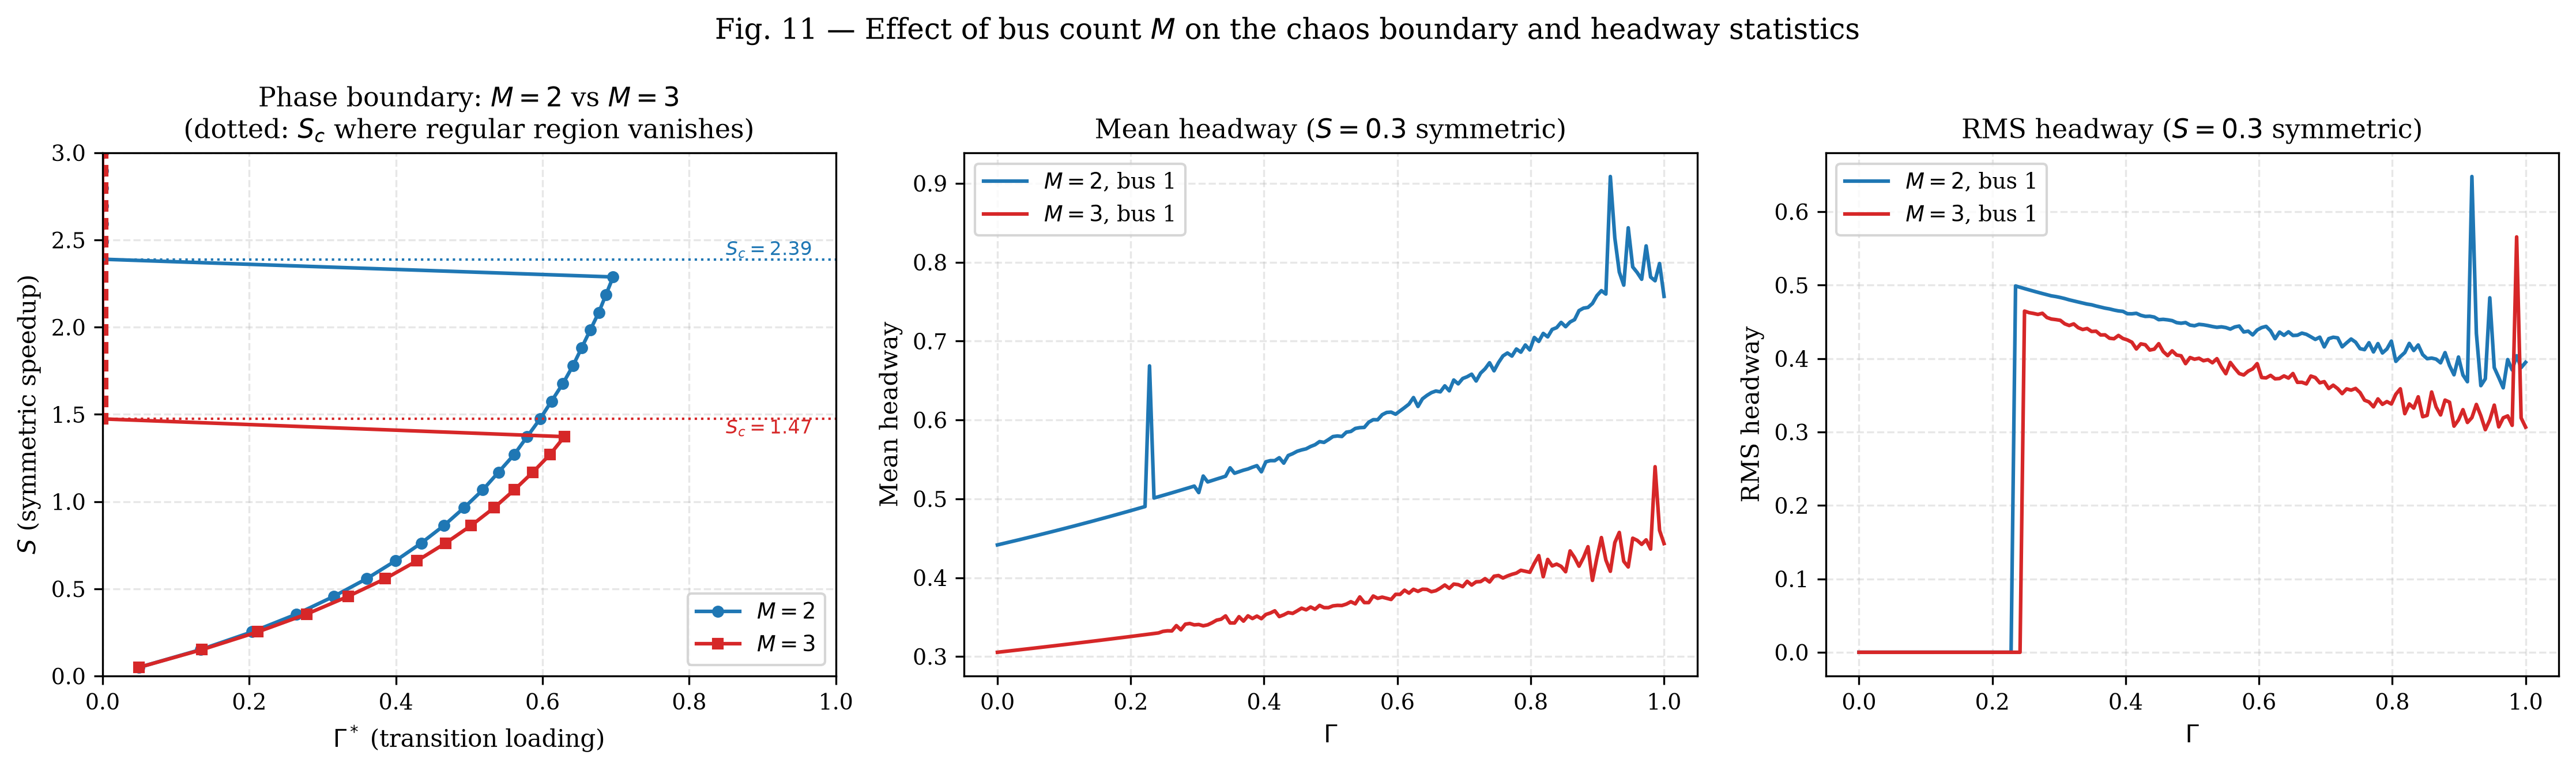
\includegraphics[width=\textwidth]{fig11_three_bus_phase.png}
		\end{column}
		\begin{column}{0.36\textwidth}
			\footnotesize
			\begin{itemize}
				\item \textbf{Left:} $\Gamma^*(S)$ for $M=2$ vs.\ $M=3$.
				\item \textbf{Centre/right:} at $S=0.3$, $M=3$ has lower mean headway (tighter route sharing) but comparable RMS onset.
				\item \alert{Headline:} bisecting on $S$ at $\Gamma=0$ finds a critical speedup $S_c$ beyond which the system is chaotic even with \emph{zero} load:
				\[
					S_c^{(2)}\approx2.39,\ \ S_c^{(3)}\approx1.47
				\]
				\item Beyond $S_c$: the speedup itself overcompensates every trip -- no loading needed.
			\end{itemize}
		\end{column}
	\end{columns}
\end{frame}

\begin{frame}{Three Buses: Takeaways}
	\footnotesize
	\setlength{\itemsep}{1pt}
	\begin{enumerate}
		\item \alert{$M=3$ generalises, not replaces, $M=2$:} same map, same algorithm, same tools -- and \emph{every} qualitative insight (period-adding bifurcations, deterministic return maps, RMS-detectable transitions) reproduces identically for $M=3$.
		\item \textbf{The transition loading $\Gamma^*$ barely moves.} A third bus delays chaos onset by under $0.005$ in $\Gamma$ at moderate symmetric speedup.
		\item \textbf{Mean headway shrinks as expected.} More buses sharing the route pack arrivals tighter -- a useful sanity check, not a new finding.
		\item \textbf{Two genuinely new effects appear only at $M\geq3$:}
		\begin{itemize}
			\item the return map becomes intrinsically two-valued in $H(m)$ alone (predecessor identity matters);
			\item the maximum useful speedup before self-induced instability drops substantially ($2.39\to1.47$).
		\end{itemize}
	\end{enumerate}

	\vspace{0.2em}
	\alert{``Just add more speedup'' is not a universal fix} -- the safety margin for that strategy shrinks as more buses are added.
\end{frame}

% =====================================================================
\useStyleHustFull
\useThinBar
\section{Interactive Demo}
% =====================================================================

\begin{frame}{Interactive Demo: Live Chaos Simulator}
	\begin{columns}[T]
		\begin{column}{0.55\textwidth}
			\centering
			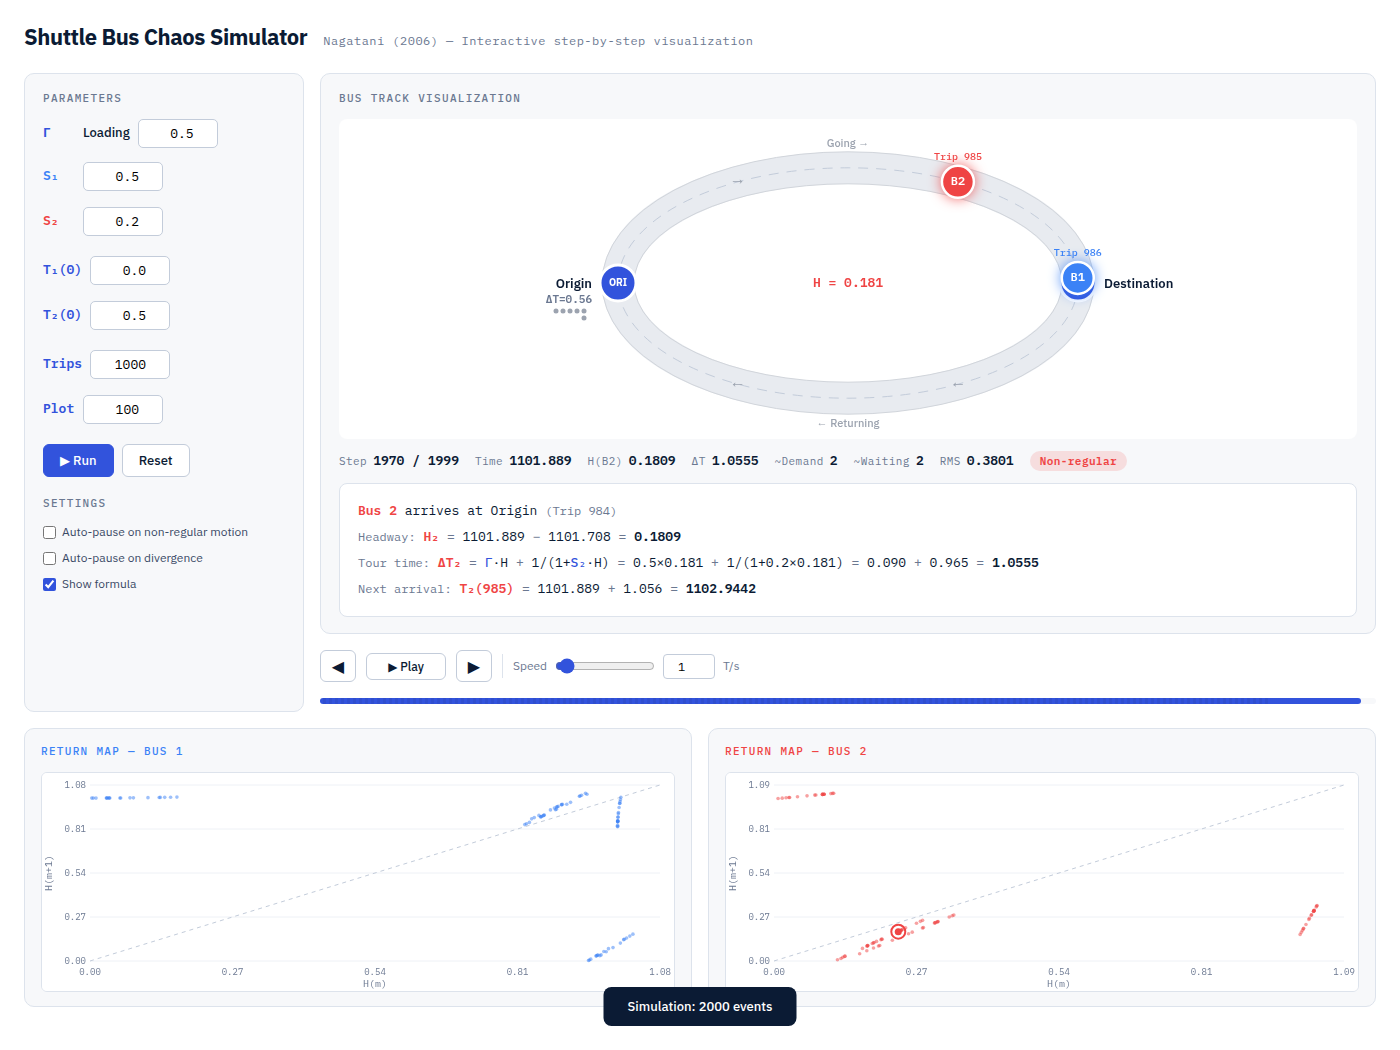
\includegraphics[width=\textwidth,height=0.72\textheight,keepaspectratio]{demo_screenshot.png}
		\end{column}
		\begin{column}{0.43\textwidth}
			\small
			\textbf{What you can do:}
			\begin{itemize}
				\item Set the number of buses $M$ (2--8), $\Gamma$, and each bus's speedup $S_i$, and watch chaos unfold step-by-step.
				\item Buses animate around the track in real time, pausing to board at the Origin and alight at the Destination.
				\item One return-map plot per bus updates live, generated dynamically for whatever $M$ is chosen.
				\item The same interface reproduces both the paper's $M=2$ figures and the $M=3$ extension just shown.
			\end{itemize}
		\end{column}
	\end{columns}
\end{frame}

% =====================================================================
\useStyleHustFull
\useThinBar
\section{Conclusion}
% =====================================================================

\begin{frame}{Conclusion}
	\footnotesize
	\setlength{\itemsep}{1pt}

	\textbf{Paper reproduction (M=2):}
	\begin{itemize}\setlength{\itemsep}{1pt}
		\item All 7 figures of Nagatani (2006) reproduced from a single event-driven simulator.
		\item Regular motion gives way to \textbf{period-adding bifurcations} ($3\to5\to7\to\cdots$), not period-doubling.
		\item Return maps reveal \textbf{deterministic structure} — chaos is governed by the nonlinear map, not randomness.
		\item Speedup $S$ delays chaos onset ($\Gamma^*$ rises with $S$), but the benefit \textbf{saturates and reverses} beyond a critical $S_c$.
	\end{itemize}

	\vspace{0.2em}
	\textbf{Extension to M=3:}
	\begin{itemize}\setlength{\itemsep}{1pt}
		\item \alert{No new model needed} — the same map (Eq.~5) and the same algorithm handle any $M$.
		\item Every qualitative insight carries over: same bifurcation route, same return-map structure, same RMS-detectable transitions.
		\item Two new effects unique to $M\geq3$: return maps become \textbf{two-valued} (predecessor identity matters); critical speedup $S_c$ drops from $\approx2.0$ to $\approx1.6$.
	\end{itemize}

	\vspace{0.15em}
	\alert{The model generalises, not just the numbers} — same equation, same code, same insights for any $M$.
\end{frame}

% =====================================================================

\hustthankyou

\end{document}
